\documentclass{article}
\usepackage[a4paper, paperwidth=25cm, paperheight=24cm, left=1.5cm, right=1.5cm, top=2cm, bottom=2cm]{geometry}
\usepackage{pgfplots}
\usepackage{tikz,tcolorbox}
\usepackage{amsmath}
\definecolor{MyBlue}{HTML}{17ADB8}
\setlength{\parindent}{0pt}

\tcbuselibrary{skins, breakable, theorems}

\newtcolorbox{prettyBox}[2]{
  enhanced,
  colback=white!90!#2,   % Background color based on the second parameter (color)
  colframe=#2!60!black,  % Frame color based on the second parameter (color)
  coltitle=white,        % Title color (white)
  fonttitle=\bfseries\Large,
  title=#1,              % Title from the first parameter
  boxrule=1mm,
  arc=0.5mm,
  drop shadow=#2!35!gray, % Drop shadow color based on the second parameter (color)
}



\begin{document}
\begin{center}
    \Huge{\textbf{\underline{Chapter 1: Introduction}}}
\end{center}

\vspace{0.35cm}


\section{Numerical Algorithm (Numerical Method)}
\begin{prettyBox}{Numerical Algorithm}{mygreen}
A Numerical Algorithm provides an approximate solution and is used to solve problems involving large amounts of data. The algorithm is based on a well-defined iterative sequence, starting with an initial solution that progressively converges toward the desired result with each iteration.

\[
\begin{cases}
    \hspace{0.1cm}(U_n) & \hspace{-0.1cm}n \geq 0 \\[0.15cm]
    \hspace{0.1cm}S_0 & \hspace{-0.3cm} \text{Initial Solution (Starting Point)}
\end{cases}
\]
\end{prettyBox}
\vspace{0.35cm}

\section{Convergence Speed (Order of Convergence)}
\begin{prettyBox}{Convergence Speed}{mygreen}
The number of iterations required to find the solution we are looking for:
\begin{itemize}
    \item Linear Order: 1 (slow)
    \item Quadratic Order: 2 (faster)
    \item \(>>\) 2 (very fast)
\end{itemize}
\end{prettyBox}

\vspace{0.35cm}

\section{Interpolation}
\begin{prettyBox}{Interpolation}{mygreen}
Estimates the value between two known points of a function allowing for a smoother representation of the function's behavior.
\end{prettyBox}

\vspace{0.35cm}

\section{Approximation}
\begin{prettyBox}{Approximation}{mygreen}
Approximates the formula of a function from a set of values, with the objective of finding a simpler function that represents the general trend of the data, even if it doesn't pass through every point exactly.
\end{prettyBox}

\vspace{0.35cm}

\section{Error}
\begin{prettyBox}{Error}{mygreen}
An error represents the difference between the actual solution and the computed result. It indicates how far we are from the true solution. There are two cases:
\begin{itemize}
    \item \textbf{Evaluation}: We know the exact solution, so we can directly calculate the error:
        \[   \boxed{E_r = |\overline{x} - x_{\text{app}}|} \]
    \item \textbf{Estimation}: We don't know the exact solution, so we only have an estimate of the error, based on the output of the algorithm:
        \[      \boxed{E_r = |\overline{x} - x_{\text{app}}| \leq \text{Algo}} \]
\end{itemize}

Where:
\begin{itemize}
    \item \(E_r\) : The error value.
    \item \(\overline{x}\) : The exact solution.
    \item \(x_{\text{app}}\) : The approximate solution.
    \item Algo : The error value found by the algorithm.
\end{itemize}
\end{prettyBox}

\vspace{0.35cm}

\section{Optimization}
\begin{prettyBox}{Optimization}{mygreen}
Optimization in numerical algorithms refers to two things:
\begin{itemize}
    \item \textbf{Error}: We aim to minimize the error in order to achieve the most accurate approximate solution.
    \item \textbf{Convergence Speed}: The higher the order of convergence, the less time the algorithm will take to converge to the solution we are looking for.
\end{itemize}
\end{prettyBox}


\section{The Birth of Software Engineering}

\subsection{Development of Hardware/Software and Their Relationship}

\begin{itemize} \item \textbf{\underline{1940-1950: Vacuum Tubes}}:
Vacuum tubes were electronic components that controlled the flow of electricity in a vacuum. Used in radios, televisions, and early computers, they were large, expensive, and consumed a lot of power, but were essential for electronics at the time.



\item \textbf{\underline{1950-1960: Transistors}}:  
Transistors are semiconductor devices used to amplify or switch electronic signals. They replaced vacuum tubes due to their smaller size, greater efficiency, and lower cost. Transistors were used in radios, early computers, and have since become fundamental in all modern electronics.

\item \textbf{\underline{1960-1970: Integrated Circuits}}:  
An integrated circuit (IC) is a small chip that contains a set of electronic circuits, including transistors, resistors, and capacitors. ICs made electronics more compact, affordable, and powerful, revolutionizing industries during the 1960s. ICs were found in computers, calculators, and a wide range of other electronic devices.

\item \textbf{\underline{1970-Present: Microprocessors}}:  
A microprocessor is a single-chip CPU (Central Processing Unit) that performs the functions of a computer's central processor. Microprocessors became more affordable in the 1970s, paving the way for the rise of personal computers, smartphones, and embedded systems in countless devices today.

\end{itemize}

\vspace{0.5cm}

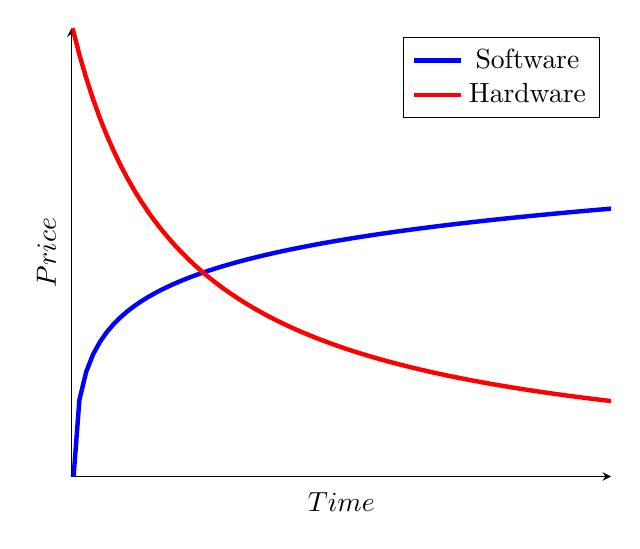
\begin{tikzpicture} \begin{axis}[ axis lines = left, xlabel=$Time$, ylabel=$Price$, domain=0.01:5, xtick=\empty, ytick=\empty, xmin=0, ymin=0, ] \addplot[ultra thick, color = blue, no marks, samples = 80] {5 + ln(0.5*x)}; \addlegendentry{Software} \addplot[ultra thick, color = red, no marks, samples = 80] {10 / (x + 1)}; \addlegendentry{Hardware} \end{axis} \end{tikzpicture}

\vspace{1.5cm}

As shown in the graph above, there is an inverse relationship between hardware and software prices. As hardware becomes more affordable and advanced, software prices tend to increase, a phenomenon often referred to as the "Software Crisis." This was primarily caused by a lack of development methodology and reflection on part of the developers. Software projects frequently went over budget, were late to release, and were often filled with bugs.

To address this issue, developers needed to establish efficient methodologies and practices for building better software.

\subsection{Qualities of Good Software}


A well-designed software product must meet several key criteria to be considered high-quality. Here are some essential qualities:

\begin{itemize}

\item \textbf{Maintainability}:
The ease with which software can be modified to correct faults, improve performance, or adapt to a changed environment. Code should be well-documented, modular, and easy to update without causing regressions in other parts of the software.


\item \textbf{Affordability}:  
High-quality software should provide value for money. The cost of development, licensing, maintenance, and support should be reasonable and aligned with the customer's budget and expectations. Affordability doesn't mean the cheapest option, but one that balances cost with features and reliability.

\item \textbf{Functionality}:  
The software must meet the specific needs of its users and perform the tasks it was designed for effectively. It should deliver all required features and capabilities, ensuring that it fulfills its purpose.

\item \textbf{Reliability}:  
Software should function consistently and accurately over time, without crashing or producing incorrect results. It should handle errors gracefully and work well under various conditions, including edge cases and unexpected inputs.

\item \textbf{Performance}:  
Good software should operate efficiently, with fast response times and minimal use of system resources. Performance includes aspects like load times, memory usage, and the ability to handle multiple tasks or large amounts of data simultaneously.

\item \textbf{Scalability}:  
The software should be able to grow and accommodate increasing amounts of work or users without a significant drop in performance. This is especially important for systems that expect long-term growth or fluctuating demand.

\item \textbf{Usability}:  
The user interface should be intuitive, making it easy for users to learn and navigate. Well-designed software provides a positive user experience, with thoughtful layouts, clear instructions, and accessible features for all users, including those with disabilities.

\item \textbf{Security}:  
Security is critical in today's environment. High-quality software should protect user data and prevent unauthorized access, ensuring compliance with security standards. It should include features like encryption, authentication, and protection against common vulnerabilities such as SQL injection or cross-site scripting.

\item \textbf{Portability}:  
Software should work across different platforms and environments with minimal modifications. This is especially important for applications intended to run on multiple operating systems, browsers, or devices. A portable software solution can save significant development effort.

\item \textbf{Interoperability}:  
High-quality software should be able to integrate and work seamlessly with other systems and tools. This includes support for standard formats, APIs, and protocols that allow it to exchange data and collaborate with other software.

\item \textbf{Minimization of Bugs}:  
A good software product should have a minimal number of defects. This involves rigorous testing during the development process to catch and fix bugs early, as well as ongoing maintenance and updates to address issues as they arise.

\item \textbf{Extensibility}:  
Software should be designed in a way that allows new features and functionality to be added in the future without significant changes to the core architecture. Extensible software can adapt to changing user needs and technology advances.

\item \textbf{Compliance with Standards}:  
High-quality software adheres to industry standards and regulations, ensuring that it meets legal, technical, and ethical guidelines. This is particularly important in industries like healthcare, finance, and government, where compliance is mandatory.
\end{itemize}

\vspace{0.5cm}

\begin{tikzpicture} \begin{axis}[ axis lines = left, xlabel=$Quality$, ylabel=$Price$, domain=0.01:5, xtick=\empty, ytick=\empty, xmin=0, ymin=0, ] \addplot[ultra thick, color = blue, no marks, samples = 80] {exp(x)}; \end{axis} \end{tikzpicture}

This graph illustrates the positive correlation between software quality and price. As the quality of the software improves, its price tends to increase exponentially.

\section{Life Cycle Of Software}
\subsection{Whats's Life Cycle Of Software?}
\subsection{WaterFall Life Cycle}

\section{Needs Analysis}
A thorough needs analysis is critical in software development. Any ambiguity, contradiction, or missing information found in the
requirements document can lead to significant setbacks, potentially requiring a restart of the project. In this section, we will
take a detailed look at how the requirements document is structured.
\begin{tcolorbox}[title = Note] 
\textbf{Difference Between Goals \& Needs ?}\\

It is crucial to understand that the requirements document holds the client's needs and not their goals . A goal is subjective and
open to interpretation, while a need is objective—measurable or verifiable.\\

\textbf{\underline{Example :}}\\

The client might request a "pleasant user interface" , This can be interpreted in many ways:
\begin{itemize}
    \item a visually appealing UI with lots of colors and animations   
    \item an easy-to-use interface
    \item a minimalistic design
\end{itemize} 

and so on. To turn this into a clear need, we must clarify what the client means. For instance, they might want the UI to be 
organized with all features accessible through a dropdown menu.

\end{tcolorbox}\subsection{Requirments Document Structure}
\begin{itemize}
   \item \textbf{Introduction : }This section provides an overview of the document by outlining its key components :
      \begin{itemize} 
          \item Purpose: The reason for creating this document, which is primarily to align the development team and facilitate
           communication with the client.
           \vspace{0.15cm}
          \item Scope: A high-level summary of the software’s main functionality, without going into too much detail. 
           \vspace{0.15cm}
          \item Context: The reason for creating the software, which could be to sell it to a client or company, to develop an
          open-source project, or other similar motivations.\\
      \end{itemize}    
    \item \textbf{Hardware : }This section states whether the software requires any special hardware components like : GPU,
sensors, or a camera ...etc . It also outlines the minimum hardware requirements needed to run the software, as well as the optimal hardware configuration for the best and smoothest experience.
    \item \textbf{Conceptual Model : }This section describes the overall software architecture through a high-level graphical
        representation, highlighting key components and their relationships.\hspace{0.1cm}It provides an overview of how the system is structured and
operates, making it easier for stakeholders to understand.

\textbf{\underline{Example :}}

A desktop system composed of an email service, a spreadsheet, a document processing service, and an information retrieval service.
\end{itemize}
\begin{center}
\begin{tikzpicture}
    \draw (0,0) rectangle (2,1);
    \node at (1,0.5){User};
    \draw[->] (1,1) -- (1,2) -- (10.5 ,2) -- (10.5,-2);
    \draw[->] (2,0.5) -- (6.25,0.5) -- (6.25,0);
    \draw[->] (0,0.5) -- (-1.5,0.5) -- (-1.5,-8) -- (1.75,-8) -- (1.75,-7);
    \draw[->] (1.625,0) -- (1.625,-1);

    \draw (0.5,-3) rectangle (2.75,-1);
    \node at (1.625,-1.75) {Email};
    \node at (1.625 ,-2.25){Management};
    \draw[->] (1.625,-3) -- (1.625,-4);
    \draw[->] (0.5,-2) -- (-0.5,-2) -- (-0.5,-6.5) -- (0.75,-6.5);
    \draw[->] (2.75,-2) -- (4.125,-2) -- (4.125,-1) -- (5.25,-1);

    \draw (0.75,-5) rectangle (2.75,-4);
    \node at (1.75,-4.5) {Network};

    \draw (0.75,-7) rectangle (2.75,-6);
    \node at (1.75,-6.5) {Spreadsheet};
    \draw[->] (2.75,-6.5) -- (5.25,-6.5);
      
    \draw (5.25,-7) rectangle (7.25,-6);
    \node at (6.25,-6.5) {DB};

    \draw(5.25,-2) rectangle (7.25,0);
    \node at (6.25,-0.75) {Document};
    \node at (6.25,-1.25) {Processing};
    \draw[->] (6.25,-2) -- (6.25,-6); 
  
    \draw (9.5,-4) rectangle (11.5,-2);
    \node at (10.5,-2.75) {Information};
    \node at (10.5,-3.25) {Retrieval};
    \draw[->] (10.5 , -4) -- (10.5,-6.5) -- (7.25,-6.5); 

 \end{tikzpicture}
\end{center}

\vspace{0.75cm}
The next step consist into creating a new conceptual model for each complexe fonction
\vspace{0.25cm}
\begin{center}
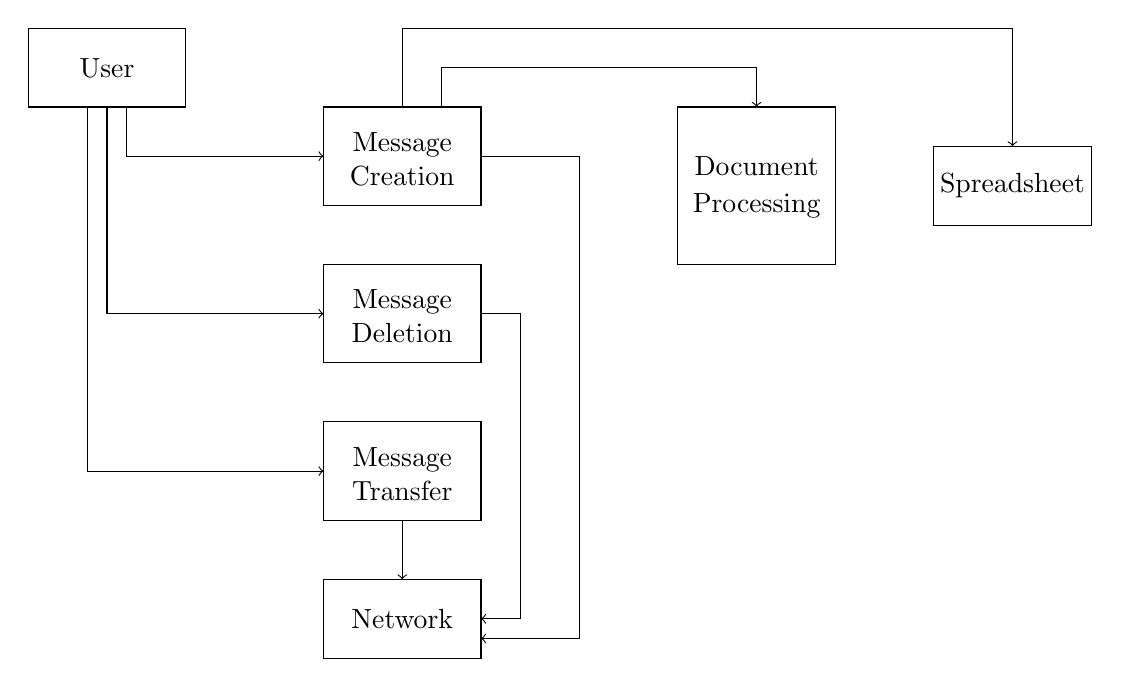
\begin{tikzpicture}
    \draw (-3,0) rectangle (-1,1);
    \node at (-2,0.5){User};
    \draw[->] (-2,0) -- (-2,-2.625) -- (0.75,-2.625);
    \draw[->] (-1.75,0) -- (-1.75,-0.625) -- (0.75,-0.625);
    \draw[->] (-2.25,0) -- (-2.25,-4.625) -- (0.75,-4.625);
    
    \draw (0.75,-1.25) rectangle (2.75,0);
    \node at (1.75,-0.475){Message};
    \node at (1.75,-0.875){Creation};
    \draw[->] (2.75,-0.625) -- (4,-0.625) -- (4,-6.75) -- (2.75,-6.75);
    \draw[->] (2.25,0) -- (2.25,0.5) -- (6.25,0.5) -- (6.25,0);
    \draw[->] (1.75,0) -- (1.75,1) -- (9.5,1) -- (9.5,-0.5);

    \draw (0.75,-3.25) rectangle (2.75,-2);
    \node at (1.75,-2.475){Message};
    \node at (1.75,-2.875){Deletion};
    \draw[->] (2.75,-2.625) -- (3.25 ,-2.625) -- (3.25,-6.5) -- (2.75,-6.5);

    \draw (0.75,-5.25) rectangle (2.75,-4);
    \node at (1.75,-4.475){Message};
    \node at (1.75,-4.875){Transfer};
    \draw[->] (1.75,-5.25) -- (1.75,-6);

    \draw (0.75,-7) rectangle (2.75,-6);
    \node at (1.75,-6.5) {Network};

    \draw (8.5,-1.5) rectangle (10.5,-0.5);
    \node at (9.5,-1) {Spreadsheet};
    
    \draw(5.25,-2) rectangle (7.25,0);
    \node at (6.25,-0.75) {Document};
    \node at (6.25,-1.25) {Processing};

\end{tikzpicture}

\end{center}
\begin{itemize}
\item \textbf{Functional Requirements:} These define what the system should do, focusing on the specific features and functions the
software must deliver to meet user or business needs. They describe the expected behavior of the system in various situations.
Functional requirements are concrete and measurable. They can be expressed using natural, semi-formal, or formal language,
or a mix of these. 

\begin{itemize} 
\item \textbf{Natural Language:} Easy to implement and understand, but lacks structure and precision, which can lead to ambiguity.
It makes automating analysis of the document harder, relying heavily on the writer’s linguistic experience. 
\item \textbf{Structured (Semi-Formal) Language:} Limited use of natural language, more structured and precise than natural language
, often accompanied by graphical notations. 
\item \textbf{Formal Language:} Hard to master and time-consuming to implement. It is difficult for clients to understand but is based
on mathematical theory, making it the most precise language and easier to automate verification. 
\end{itemize}

\item \textbf{Non-Functional Requirements:} Define the restrictions and constraints related to both hardware and software within
the context of the ongoing project. Non-functional requirements are particularly influenced by changes in technologies 
(both hardware and software) and are crucial for complex software systems. As the project develops, changes in hardware may occur.
These changes can be anticipated by projecting the expected performance levels that will be required by the end of the project.
\item \textbf{Maintenance Information:} Anticipates possible actions after the software's initial release, such as adding
new features, improving performance, or addressing potential issues.
   \item \textbf{Glossary:} Provides definitions of the terms and concepts used in the document to help readers. This ensures
that the terminology is clear, as the requirements document is shared and read by the design team, developers, and stakeholders, 
without assuming prior knowledge of these terms.
  \item \textbf{Index:} Helps the reader find specific topics and sections of the document more efficiently by providing a
detailed list of references to relevant sections, parts, and page numbers.
\end{itemize}
\begin{tcolorbox}[title = Note]
 Functional and non-functional requirements are inherently connected, and their interplay can sometimes lead to conflicts. 
 By understanding the potential for these conflicts and establishing a process for managing them, development teams can better
 balance user needs and system performance, ultimately leading to a more successful product.
\end{tcolorbox}

\subsection{Requirements Validation}
The requirements need to be coherent, realizable, and complete. Anticipation of hardware needs to be considered. 
It is crucial for the requirements document to be validated in order to initiate the next steps of the software life cycle.

\begin{itemize}
    \item review Technique is an efficient way to monitor and update the requirements .
    \item There are various analysis tools available that can facilitate the validation process of the requirements document,
helping to ensure accuracy and completeness.
\end{itemize}


\section{UML}
\subsection{Introduction}
As seen in the previous sections, the requirements document is very important, as any mistake, ambiguity,
or misunderstanding of the client's needs can lead to a project restart. We've reviewed the high-level
structure of a requirements document; one of the most important parts is the functional requirements, which can
be expressed in natural language. This approach is easy to implement and understand but isn't very precise, doesn't
automate verification, and relies solely on the linguistic experience of the writer. There is also a formal approach
based on mathematical theory, which automates verification, is very precise, but is hard to master and 
time-consuming. Finally, there is a semi-formal approach that benefits from the advantages of both natural and 
formal language; an example of this is UML (Unified Modeling Language).
\subsection{UML(Unified Modeling Language)}
UML is a semi-formal language that is easy to understand and widely used by developers. It divides into two main categories of diagrams:
\begin{itemize}
    \item Structure Diagram : Represent the static aspects of a system, showing its classes, objects, and relationships. 
    \item Behaviour Diagram :  Describes the dynamic aspects of a system, illustrating how actors interact with the system and how the system changes over time.
\end{itemize}
In this section we will focus on Use case diagram
\begin{center}
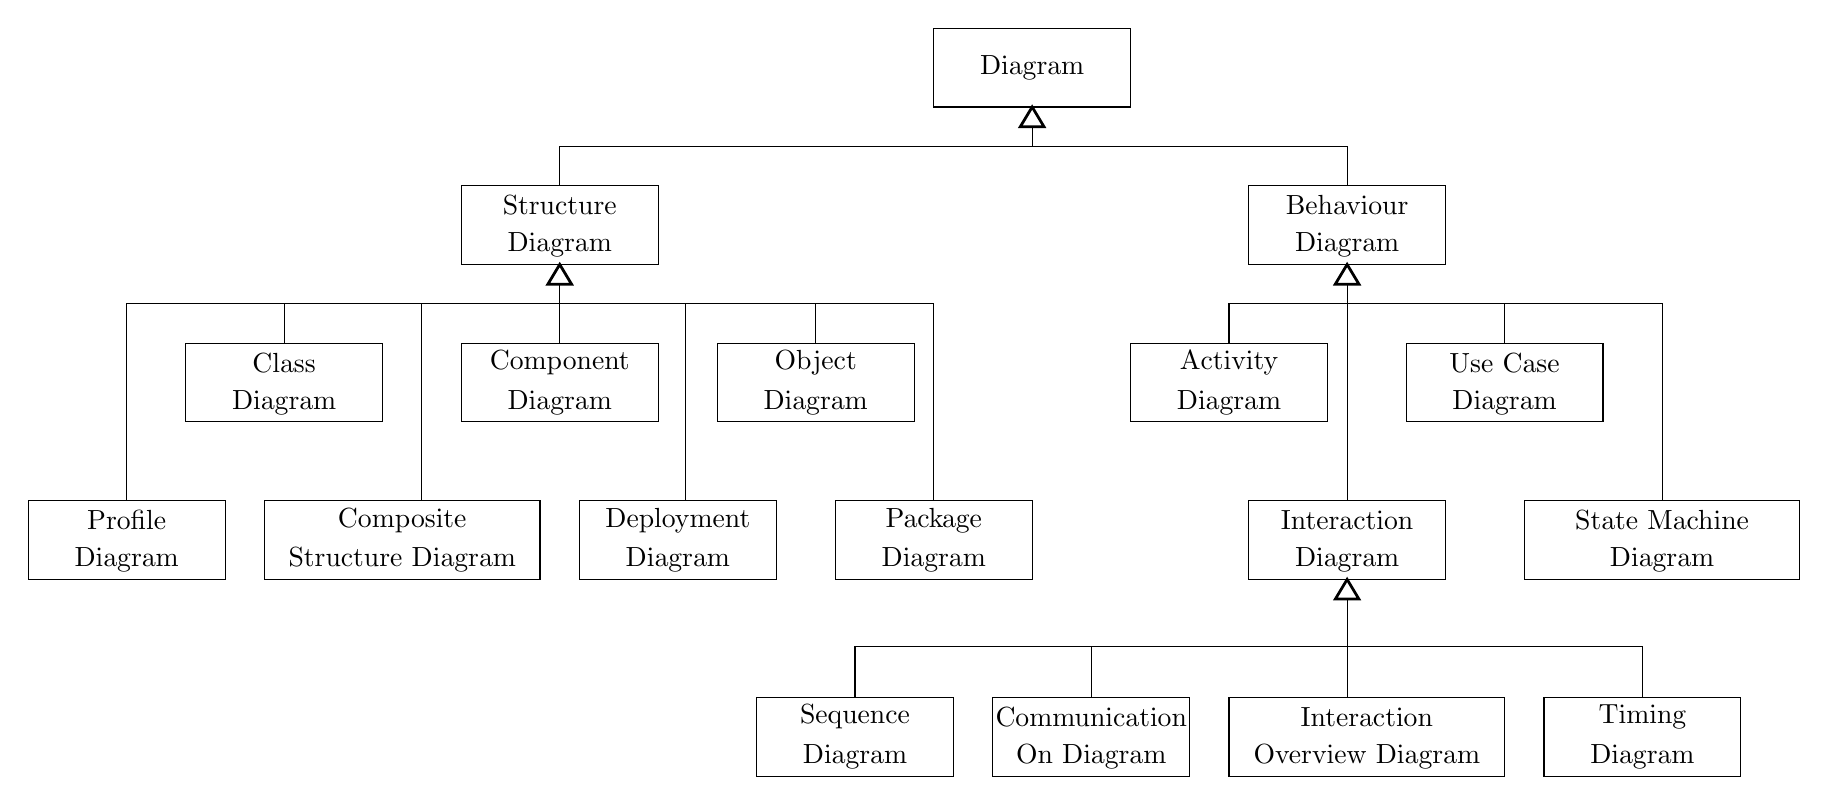
\begin{tikzpicture}
    \draw(0,0) rectangle(2.5,1);
    \node at(1.25,0.5) {Diagram};
    
    \coordinate (A) at (1.25,0);  
    \coordinate (B) at (1.1,-0.25);  
    \coordinate (C) at (1.4,-0.25);
    \draw[line width=1pt] (A) -- (B) -- (C) -- cycle;
    
    \draw (1.25,-0.25) -- (1.25,-0.5);
    \draw (-4.75,-1) -- (-4.75,-0.5) -- (5.25,-0.5) -- (5.25,-1);

    \draw(-6,-2) rectangle(-3.5,-1);
    \node at (-4.75,-1.25){Structure};
    \node at (-4.75,-1.75){Diagram};
   
    \coordinate (A) at (-4.75,-2);  
    \coordinate (B) at (-4.9,-2.25);  
    \coordinate (C) at (-4.6,-2.25);
    \draw[line width=1pt] (A) -- (B) -- (C) -- cycle;
   
    \draw (-4.75,-2.25) -- (-4.75,-3);
    \draw (-10.25,-5) -- (-10.25,-2.5) -- (0,-2.5) -- (0,-5);

    \draw (-6,-4) rectangle(-3.5,-3);
    \node at (-4.75,-3.25){Component};
    \node at (-4.75,-3.75){Diagram};
    \draw (-4.75,-3) -- (-4.75,-2.5);
    
    \draw (-9.5,-4) rectangle(-7,-3);
    \node at (-8.25,-3.25){Class};
    \node at (-8.25,-3.75){Diagram};
    \draw (-8.25,-3) -- (-8.25,-2.5);
 
    \draw (-2.75,-4) rectangle(-0.25,-3);
    \node at (-1.5,-3.25){Object};
    \node at (-1.5,-3.75){Diagram};
    \draw (-1.5,-3) -- (-1.5,-2.5);
    
    \draw (-11.5,-6) rectangle(-9,-5);
    \node at (-10.25,-5.25){Profile};
    \node at (-10.25,-5.75){Diagram};
    
    \draw (-8.5,-6) rectangle(-5,-5);
    \node at (-6.75,-5.25){Composite};
    \node at (-6.75,-5.75){Structure Diagram};
    \draw (-6.5,-5) -- (-6.5,-2.5);

    \draw (-4.5,-6) rectangle(-2,-5);
    \node at (-3.25,-5.25){Deployment};
    \node at (-3.25,-5.75){Diagram};
    \draw (-3.15,-5) -- (-3.15,-2.5);
    
    \draw (-1.25,-6) rectangle(1.25,-5);
    \node at (0,-5.25){Package};
    \node at (0,-5.75){Diagram};

    \draw(4,-2) rectangle(6.5,-1);
    \node at (5.25,-1.25){Behaviour};
    \node at (5.25,-1.75){Diagram};

    \coordinate (A) at (5.25,-2);  
    \coordinate (B) at (5.1,-2.25);  
    \coordinate (C) at (5.4,-2.25);
    \draw[line width=1pt] (A) -- (B) -- (C) -- cycle;
    
    \draw (2.5,-4) rectangle(5,-3);
    \node at (3.75,-3.25){Activity};
    \node at (3.75,-3.75){Diagram};
   
    \draw  (3.75,-3)--(3.75,-2.5)--(9.25,-2.5)--(9.25,-5);

    \draw (6,-4) rectangle(8.5,-3);
    \node at (7.25,-3.25){Use Case};
    \node at (7.25,-3.75){Diagram};
    \draw  (7.25,-3)--(7.25,-2.5);

    \draw (4,-6) rectangle(6.5,-5);
    \node at (5.25,-5.25){Interaction};
    \node at (5.25,-5.75){Diagram};
    \draw  (5.25,-5)--(5.25,-2.25);
    
    \coordinate (A) at (5.25,-6);  
    \coordinate (B) at (5.1,-6.25);  
    \coordinate (C) at (5.4,-6.25);
    \draw[line width=1pt] (A) -- (B) -- (C) -- cycle;
    
    \draw (7.5,-6) rectangle(11,-5);
    \node at (9.25,-5.25){State Machine};
    \node at (9.25,-5.75){Diagram};

    \draw (3.75,-8.5) rectangle(7.25,-7.5);
    \node at (5.5,-7.75){Interaction};
    \node at (5.5,-8.25){Overview Diagram};
    \draw  (5.25,-7.5)--(5.25,-6.25);
    
    \draw (7.75,-8.5) rectangle(10.25,-7.5);
    \node at (9,-7.75){Timing};
    \node at (9,-8.25){Diagram};

    \draw (0.75,-8.5) rectangle(3.25,-7.5);
    \node at (2,-7.75){Communication};
    \node at (2,-8.25){On Diagram};
    \draw  (2,-7.5)--(2,-6.85);
    
    \draw (-2.25,-8.5) rectangle(0.25,-7.5);
    \node at (-1,-7.75){Sequence};
    \node at (-1,-8.25){Diagram};

    \draw (-1,-7.5)--(-1,-6.85)--(9,-6.85)--(9,-7.5);
\end{tikzpicture}
\end{center}
\vspace{2cm}


\subsection{Use Case Diagram}
A use case diagram is a graphical representation of a behavior diagram, composed of three elements:

\begin{itemize} 
    \item Actors: Actors interact with the software and can have one or multiple roles. They are represented as
stick figures and may be: 
        \begin{itemize} 
            \item Human: 
              \begin{itemize} 
                \item Internal: People inside the company, such as employees, finance staff, and legal personnel.
                \item External: People outside of the company, such as end-users or customers. 
              \end{itemize} 
            \item Non-Human: Hardware (e.g., sensors, cameras) or other software systems (e.g., APIs, DBMS) that 
interact with the project’ssoftware. 
      \end{itemize} 
   \item Use Cases (Features): These represent features or functions of the software and are shown as ellipses.
   \item Associations: Associations are the connections between actors and use cases, represented with lines. 
\end{itemize}

\vspace{0.5cm}
\subsubsection*{\underline{Example:}}

\vspace{0.5cm}
\begin{center}
    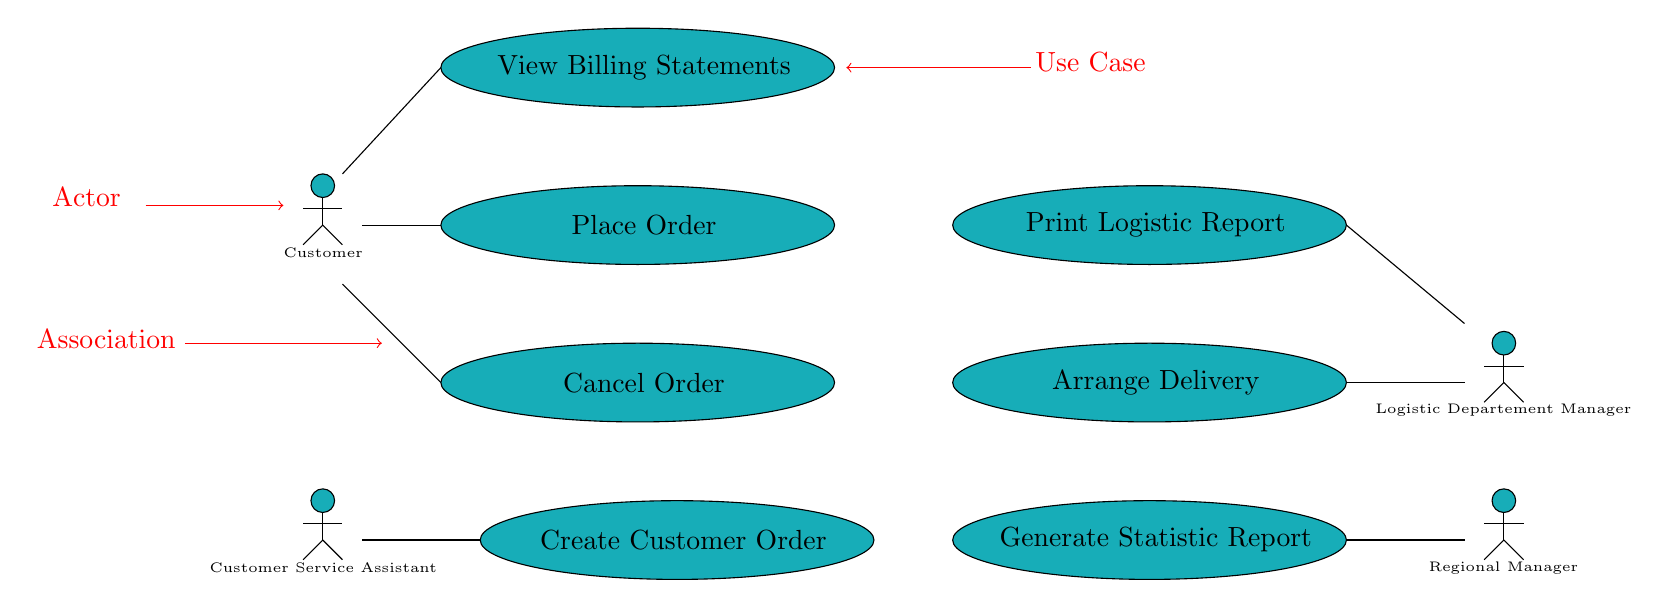
\begin{tikzpicture}

        \draw[->, red] (-6.25,-1.75) -- (-4.5,-1.75);
        \node at (-7,-1.65){\textcolor{red}{Actor}};
        \draw[->, red] (-5.75,-3.5) -- (-3.25,-3.5);
        \node at (-6.75,-3.45){\textcolor{red}{Association}};
        \draw[<-,red] (2.65,0) -- (5,0);
        \node at (5.75,0.07){\textcolor{red}{Use Case}};
        
        \fill[MyBlue] (-4,-1.5) circle(0.15);
        \draw (-4,-1.5) circle(0.15);
        \draw (-4,-1.65)--(-4,-2);
        \draw (-4.25,-1.795)--(-3.75,-1.795);
        \draw (-4,-2) -- (-3.75,-2.25);
        \draw (-4,-2) -- (-4.25,-2.25);
        \node at (-3.995,-2.35){\tiny Customer};

        \draw (-3.75,-1.35) -- (-2.5,0);
        \fill[MyBlue] (0,0) ellipse (2.5 and 0.5);
        \draw (0,0) ellipse (2.5 and 0.5);
        \node at(0.08,0){View Billing Statements};


        \draw (-3.5,-2) -- (-2.5,-2);
        \fill[MyBlue] (0,-2) ellipse (2.5 and 0.5);
        \draw (0,-2) ellipse (2.5 and 0.5);
        \node at(0.08,-2){Place Order};


        \draw (-3.75,-2.75) -- (-2.5,-4);
        \fill[MyBlue] (0,-4) ellipse (2.5 and 0.5);
        \draw (0,-4) ellipse (2.5 and 0.5);
        \node at(0.08,-4){Cancel Order};

        \fill[MyBlue] (-4,-5.5) circle(0.15);
        \draw (-4,-5.5) circle(0.15);
        \draw (-4,-5.65)--(-4,-6);
        \draw (-4.25,-5.795)--(-3.75,-5.795);
        \draw (-4,-6) -- (-3.75,-6.25);
        \draw (-4,-6) -- (-4.25,-6.25);
        \node at (-3.995,-6.35){\tiny Customer Service Assistant};
        
        \fill[MyBlue] (0.5,-6) ellipse (2.5 and 0.5);
        \draw (0.5,-6) ellipse (2.5 and 0.5);
        \draw (-3.5,-6) -- (-2,-6);
        \node at(0.58,-6){Create Customer Order};
 
        \fill[MyBlue] (11,-5.5) circle(0.15);
        \draw (11,-5.5) circle(0.15);
        \draw (11,-5.65)--(11,-6);
        \draw (10.75,-5.795)--(11.25,-5.795);
        \draw (11,-6) -- (11.25,-6.25);
        \draw (11,-6) -- (10.75,-6.25);
        \node at (10.995,-6.35){\tiny Regional Manager};
       

        \draw (9,-6) -- (10.5,-6);
        \fill[MyBlue] (6.5,-6) ellipse (2.5 and 0.5);
        \draw (6.5,-6) ellipse (2.5 and 0.5);
        \node at(6.58,-6){Generate Statistic Report};


        \draw (9,-4) -- (10.5,-4);
        \fill[MyBlue] (6.5,-4) ellipse (2.5 and 0.5);
        \draw (6.5,-4) ellipse (2.5 and 0.5);
        \node at(6.58,-4){Arrange Delivery};


        \draw (9,-2) -- (10.5,-3.25);
        \fill[MyBlue] (6.5,-2) ellipse (2.5 and 0.5);
        \draw (6.5,-2) ellipse (2.5 and 0.5);
        \node at(6.58,-2){Print Logistic Report};

        \fill[MyBlue] (11,-3.5) circle(0.15);
        \draw (11,-3.5) circle(0.15);
        \draw (11,-3.65)--(11,-4);
        \draw (10.75,-3.795)--(11.25,-3.795);
        \draw (11,-4) -- (11.25,-4.25);
        \draw (11,-4) -- (10.75,-4.25);

        \node at (10.995,-4.35){\tiny Logistic Departement Manager};

    \end{tikzpicture}
\end{center}

\vspace{1.5cm}
\newpage
\subsubsection{Relations In User Case Diagram}
\begin{itemize}
    \item  \textbf{Generalization}:  Generalization establishes a hierarchical relationship that helps organize
actors and use cases in UML diagrams. 
        \begin{itemize}
            \item  \textbf{Between Actors}: When a child actor is linked to a parent actor, it inherits all the roles and
responsibilities of the parent actor,in addition to its own specific roles. This helps clarify who can perform
what actions in the system.

\vspace{0.35cm}
\begin{center}
       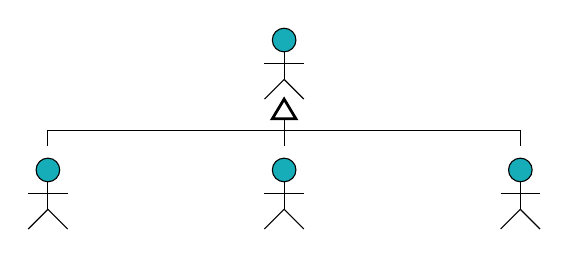
\begin{tikzpicture}
        \fill[MyBlue] (-4,-1.5) circle(0.15);
        \draw (-4,-1.5) circle(0.15);
        \draw (-4,-1.65)--(-4,-2);
        \draw (-4.25,-1.795)--(-3.75,-1.795);
        \draw (-4,-2) -- (-3.75,-2.25);
        \draw (-4,-2) -- (-4.25,-2.25);
   

        \coordinate (A) at (-4,-2.25);  
        \coordinate (B) at (-4.15,-2.5);  
        \coordinate (C) at (-3.85,-2.5);
        \draw[line width=1pt] (A) -- (B) -- (C) -- cycle;

        \fill[MyBlue] (-4,-3.15) circle(0.15);
        \draw (-4,-3.15) circle(0.15);
        \draw (-4,-3.3)--(-4,-3.65);
        \draw (-4.25,-3.445)--(-3.75,-3.445);
        \draw (-4,-3.65) -- (-3.75,-3.9);
        \draw (-4,-3.65) -- (-4.25,-3.9); 

        \fill[MyBlue] (-7,-3.15) circle(0.15);
        \draw (-7,-3.15) circle(0.15);
        \draw (-7,-3.3)--(-7,-3.65);
        \draw (-7.25,-3.445)--(-6.75,-3.445);
        \draw (-7,-3.65) -- (-6.75,-3.9);
        \draw (-7,-3.65) -- (-7.25,-3.9);

        \fill[MyBlue] (-1,-3.15) circle(0.15);
        \draw (-1,-3.15) circle(0.15);
        \draw (-1,-3.3)--(-1,-3.65);
        \draw (-1.25,-3.445)--(-0.75,-3.445);
        \draw (-1,-3.65) -- (-0.75,-3.9);
        \draw (-1,-3.65) -- (-1.25,-3.9);

        \draw (-7,-2.85)--(-7,-2.65) -- (-1,-2.65) -- (-1,-2.85);
        \draw (-4,-2.5)--(-4,-2.85);

    \end{tikzpicture} 
\end{center}


\vspace{0.35cm}

            \item  \textbf{Between Use Cases}: Allows a feature to be divided into multiple, more specific
versions. These child use cases represent the same general feature but can differ in their implementation or method.
This promotes reusability and clarity in how features are handled in different scenarios.
        \end{itemize}

\vspace{0.35cm}
        \begin{center}
            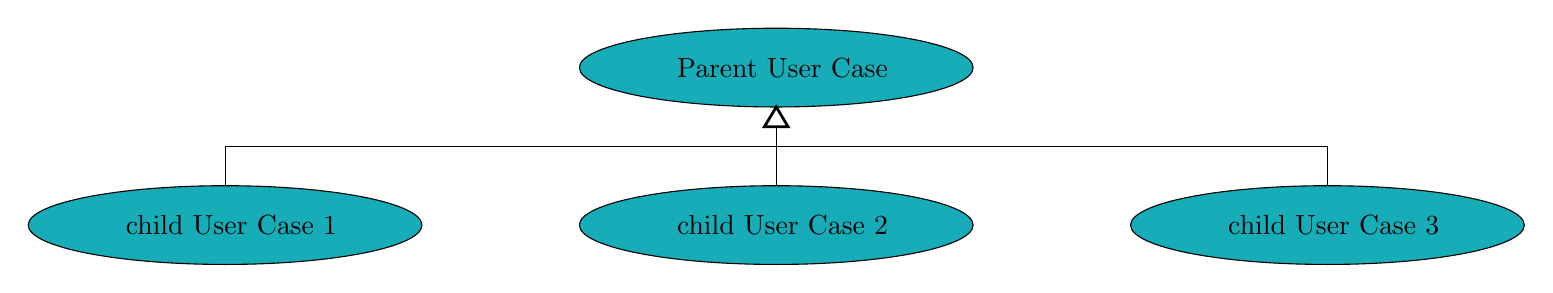
\begin{tikzpicture}
            \fill[MyBlue] (0,0) ellipse (2.5 and 0.5);
            \draw (0,0) ellipse (2.5 and 0.5);
            \node at (0.08,0) {Parent User Case};
        
        \coordinate (A) at (0,-0.5);  
        \coordinate (B) at (-0.15,-0.75);  
        \coordinate (C) at (0.15,-0.75);
        \draw[line width=1pt] (A) -- (B) -- (C) -- cycle;
        
           \fill[MyBlue] (0,-2) ellipse (2.5 and 0.5);
            \draw (0,-2) ellipse (2.5 and 0.5);
            \node at (0.08,-2) {child User Case 2};
            
            \fill[MyBlue] (7,-2) ellipse (2.5 and 0.5);
            \draw (7,-2) ellipse (2.5 and 0.5);
            \node at (7.08,-2) {child User Case 3};

            \fill[MyBlue] (-7,-2) ellipse (2.5 and 0.5);
            \draw (-7,-2) ellipse (2.5 and 0.5);
            \node at (-6.92,-2) {child User Case 1};

            \draw (-7,-1.5) -- (-7,-1) -- (7,-1) -- (7,-1.5);
            \draw (0,-1.5) -- (0,-0.75);
            \end{tikzpicture}
        \end{center}
          

\vspace{0.35cm}

    \item  \textbf{Inclusion}: This relationship applies only between use cases. The destination use case 
must execute before  the source use case whenever the source use case is invoked. 
 
\vspace{0.35cm}
        \begin{center}
            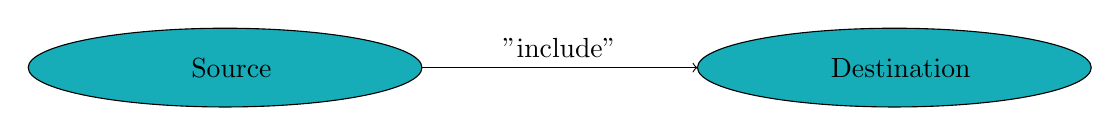
\begin{tikzpicture}
                
            \fill[MyBlue] (-2,0) ellipse (2.5 and 0.5);
            \draw (-2,0) ellipse (2.5 and 0.5);
            \node at (-1.92,0){Source};
            
            \draw[->] (0.5,0)--(4,0);
            \node at (2.25,0.25){"include"};

            \fill[MyBlue] (6.5,0) ellipse (2.5 and 0.5);
            \draw (6.5,0) ellipse (2.5 and 0.5);
            \node at (6.58,0){Destination};
            \end{tikzpicture}
    \end{center}
    

\vspace{0.35cm}
\item  \textbf{Extension}: This relationship applies only between use cases. Before executing the destination use case, 
a specific condition is checked. If the condition is met, the source use case will execute
before the destination use case.
 
\vspace{0.35cm}
\begin{center}
            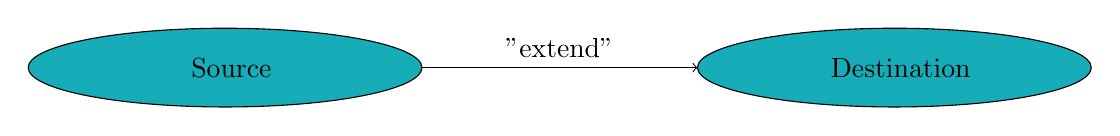
\begin{tikzpicture}
                
            \fill[MyBlue] (-2,0) ellipse (2.5 and 0.5);
            \draw (-2,0) ellipse (2.5 and 0.5);
            \node at (-1.92,0){Source};
            
            \draw[->] (0.5,0)--(4,0);
            \node at (2.25,0.25){"extend"};

            \fill[MyBlue] (6.5,0) ellipse (2.5 and 0.5);
            \draw (6.5,0) ellipse (2.5 and 0.5);
            \node at (6.58,0){Destination};
            \end{tikzpicture}
    \end{center}

\end{itemize}


\subsubsection*{\underline{Example:}}
Let's Take the example of a bank application\\\\ 
\textbf{\underline{Generalisation Between Use Cases:}}

\vspace{0.25cm}
the diagram below shows a generalisation relationship between use case 
where the main feature is transfert that is divided into specific method and way of achieving the transfert (ATM,Manual,Online)
\vspace{0.5cm}
\begin{center}
            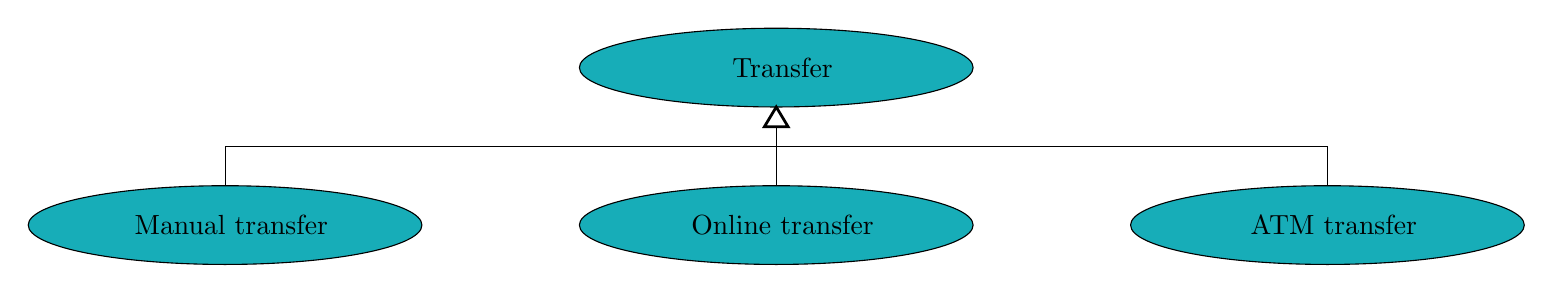
\begin{tikzpicture}
            \fill[MyBlue] (0,0) ellipse (2.5 and 0.5);
            \draw (0,0) ellipse (2.5 and 0.5);
            \node at (0.08,0) {Transfer};
        
        \coordinate (A) at (0,-0.5);  
        \coordinate (B) at (-0.15,-0.75);  
        \coordinate (C) at (0.15,-0.75);
        \draw[line width=1pt] (A) -- (B) -- (C) -- cycle;
        
           \fill[MyBlue] (0,-2) ellipse (2.5 and 0.5);
            \draw (0,-2) ellipse (2.5 and 0.5);
            \node at (0.08,-2) {Online transfer};
            
            \fill[MyBlue] (7,-2) ellipse (2.5 and 0.5);
            \draw (7,-2) ellipse (2.5 and 0.5);
            \node at (7.08,-2) {ATM transfer};

            \fill[MyBlue] (-7,-2) ellipse (2.5 and 0.5);
            \draw (-7,-2) ellipse (2.5 and 0.5);
            \node at (-6.92,-2) {Manual transfer};

            \draw (-7,-1.5) -- (-7,-1) -- (7,-1) -- (7,-1.5);
            \draw (0,-1.5) -- (0,-0.75);
            \end{tikzpicture}
        \end{center}


        \vspace{1cm}

\textbf{\underline{Generalisation Between Actors:}}

\vspace{0.25cm}
the diagram below shows a generalisation relationship between Actors where the child actor Service Manager 
is inheriting all roles of the parent actor teller + his own roles

\vspace{0.15cm}

\begin{center}
       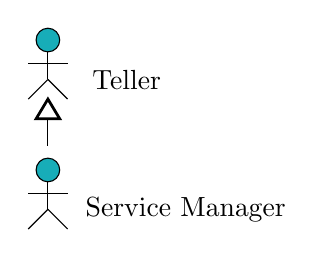
\begin{tikzpicture}
        \fill[MyBlue] (-4,-1.5) circle(0.15);
        \draw (-4,-1.5) circle(0.15);
        \draw (-4,-1.65)--(-4,-2);
        \draw (-4.25,-1.795)--(-3.75,-1.795);
        \draw (-4,-2) -- (-3.75,-2.25);
        \draw (-4,-2) -- (-4.25,-2.25);
        \node at (-3,-2){Teller};


        \coordinate (A) at (-4,-2.25);  
        \coordinate (B) at (-4.15,-2.5);  
        \coordinate (C) at (-3.85,-2.5);
        \draw[line width=1pt] (A) -- (B) -- (C) -- cycle;

        \fill[MyBlue] (-4,-3.15) circle(0.15);
        \draw (-4,-3.15) circle(0.15);
        \draw (-4,-3.3)--(-4,-3.65);
        \draw (-4.25,-3.445)--(-3.75,-3.445);
        \draw (-4,-3.65) -- (-3.75,-3.9);
        \draw (-4,-3.65) -- (-4.25,-3.9); 
        \node at (-2.25,-3.65){Service Manager};
        
        \draw (-4,-2.5)--(-4,-2.85);
    \end{tikzpicture}
\end{center}

        \vspace{1cm}
\textbf{\underline{inclusion Between Use Cases:}}

\vspace{0.25cm}
the diagram below shows an inclusion relationship between use cases where each time the transfert case is invoked
the identification case must execute first 

\vspace{0.15cm}

        \begin{center}
            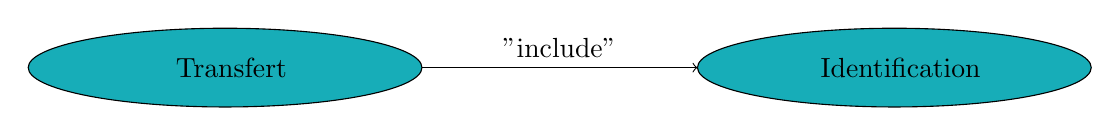
\begin{tikzpicture}
                
            \fill[MyBlue] (-2,0) ellipse (2.5 and 0.5);
            \draw (-2,0) ellipse (2.5 and 0.5);
            \node at (-1.92,0){Transfert};
            
            \draw[->] (0.5,0)--(4,0);
            \node at (2.25,0.25){"include"};

            \fill[MyBlue] (6.5,0) ellipse (2.5 and 0.5);
            \draw (6.5,0) ellipse (2.5 and 0.5);
            \node at (6.58,0){Identification};
            \end{tikzpicture}
    \end{center}

        \vspace{1cm}
        \newpage
\textbf{\underline{Extension Between Use Cases:}}

\vspace{0.25cm}
the diagram below shows an extension relationship between use cases where each time the transfert case is invoked
the balance check case will be executed if the value is \textgreater= 10000 DA

\vspace{0.15cm}


        \begin{center}
            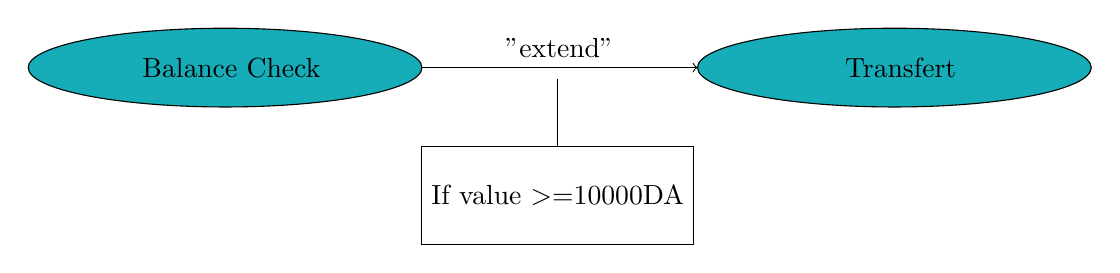
\begin{tikzpicture}
                
            \fill[MyBlue] (-2,0) ellipse (2.5 and 0.5);
            \draw (-2,0) ellipse (2.5 and 0.5);
            \node at (-1.92,0){Balance Check};
            
            \draw[->] (0.5,0)--(4,0);
            \node at (2.25,0.25){"extend"};

            \fill[MyBlue] (6.5,0) ellipse (2.5 and 0.5);
            \draw (6.5,0) ellipse (2.5 and 0.5);
            \node at (6.58,0){Transfert};

            \draw (0.5,-2.25) rectangle (3.95,-1);
            \node at (2.225,-1.625){If value \textgreater=10000DA};
            \draw (2.225,-1) -- (2.225,-0.15);
            \end{tikzpicture}
    \end{center}

        \vspace{1cm}
\begin{tcolorbox}[title = Note]
 \textbf{Difference Between Inclusion \& Extension :}\\
In The inclusion relationship the Destination case will always execute before source case in all cases , whereas
in the extension relationship the source case will execute before destination source only if certain conditions
are met

\end{tcolorbox}

\end{document}
